\documentclass[a4paper, 12pt]{article} % тип документа

%%%Библиотеки
    %\usepackage[warn]{mathtext}	
    \usepackage[T2A]{fontenc}   %Кодировка
    \usepackage[utf8]{inputenc} %Кодировка исходного текста
    \usepackage[english, russian]{babel} %Локализация и переносы
    \usepackage{caption}
    \usepackage{listings}
    \usepackage{amsmath, amsfonts, amssymb, amsthm, mathtools}
    \usepackage[warn]{mathtext}
    \usepackage[mathscr]{eucal}
    \usepackage{wasysym}
    \usepackage{graphicx} %Вставка картинок правильная
    \usepackage{indentfirst}
    \usepackage{float}    %Плавающие картинки
    \usepackage{wrapfig}  %Обтекание фигур (таблиц, картинок и прочего)
    \usepackage{fancyhdr} %Загрузим пакет
    \usepackage{lscape}
    \usepackage{xcolor}
    \usepackage[normalem]{ulem}
    
    \usepackage{titlesec}
    \titlelabel{\thetitle.\quad}

    \usepackage{hyperref}

%%%Конец библиотек

%%%Настройка ссылок
    \hypersetup
    {
        colorlinks = true,
        linkcolor  = blue,
        filecolor  = magenta,
        urlcolor   = blue
    }
%%%Конец настройки ссылок


%%%Настройка колонтитулы
    \pagestyle{fancy}
    \fancyhead{}
    \fancyhead[L]{Безынерционные цепи}
    \fancyhead[R]{Глаз Роман, группа Б01-007}
    \fancyfoot[C]{\thepage}
%%%конец настройки колонтитулы

\begin{document}

\section{Параллельный сумматор}

\subsection{Подготовка}

Для работы выбраны резисторы $R_1 = 5,1$ кОм, $R_2 = 10$ кОм, тогда $R = \frac{3}{2} R_1 || R_2 = 5,066 \approx 5,1$ кОм. В этом случае $\alpha = 1,96$, $\beta = 4,04$.

\subsection{Вычисления}

Соберём следующую схему, где на $E_1$ подадим синусоидальное напряжение амплитудой 2 В, а на $E_2$ постоянно напряжение амплитудой 5 В.

\begin{figure}[h]
    \centering
    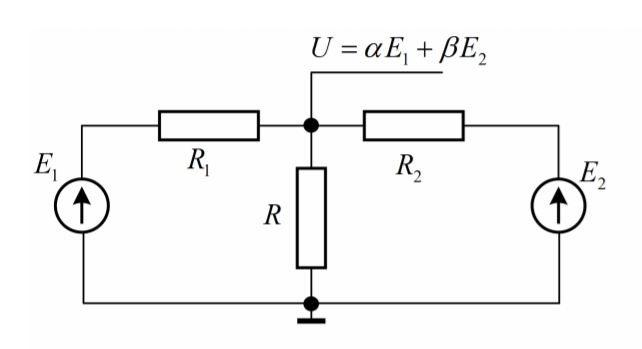
\includegraphics[width = 8 cm]{1.png}
    \caption{Параллельный сумматор}
    \label{fig:vac}
\end{figure}

В этом случае осциллограф показываем постоянную составляющую напряжения $U$ $U_{const} = 0,575$ В, амплитуда переменной составляющей равна $U_{vol} = 0,117$ В.

Подавая сигналы на первый и второй входы сумматора
поочерёдно при коротком замыкании на свободном входе, измерим коэффициенты $\alpha$ и $\beta$. 

В случае замыкания накоротко источника $E_1$ имеем $U_2 = 1,004$, для $E_2$ имеем $U_1 = 2,056$ В (в качестве напряжения источника используется $E = 5$ В). Тогда $\alpha = \frac{U_1}{E} = 0,411$, когда $\beta = \frac{U_2}{E} = 0,201$. Получили значения, почти совпадающие с теортическими. При этом $\frac{\alpha}{\beta} = 2,044 \approx 2$.

Найдём сопротивление схемы (см. Рис. 2) $R^*$. Дл этого используем метод двух нагрузок. Разорвав цепи в месте источников постоянного тока пусть напряжение $5$ В на полученную схему. При этом напряжение на выходе $U_{01} = 1,177$ В. В случае ещё одной параллельно соединённой нагрузки $R_{add} = 3,9$ кОм, имеем $U_{02} = 0,777$ В.

Тогда 
$$U_{01} = R^* \cdot I, \; U_{02} = \frac{R_{add}R^*}{R_{add} + R^*} \cdot I = \frac{U_{01}R_{add}}{R_{add} + R^*}$$

Отсюда $R^* = 1,99$ кОм.

Теоретиеское же значение сопротивления равно $R^* = R_1 || R_2 || R = 2,03$ кОм.

\begin{figure}[h!]
    \centering
    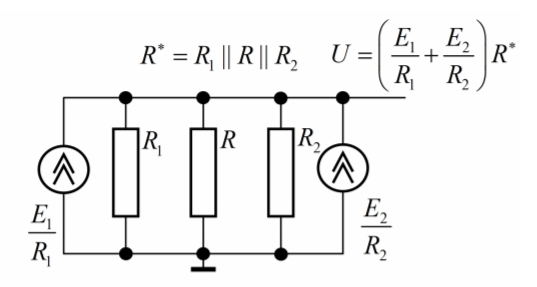
\includegraphics[width = 10 cm]{2.png}
    \caption{Эквивалетная схема}
    \label{fig:vac}
\end{figure}

\section{H-параметры}

\subsection{Проверка основной формулы}

Если $U_2 = 0$, то коэффициент $h_{11}$ очевиден: $h_{11} = R_1 + R_2 || R_3$. Аналогично $h_{21} = \frac{R_3}{R_2 + R_3}$ -- из закона Ома.

Если $I_1 = 0$, то $h_{12} = \frac{U_1}{U_2} = - \frac{R_3}{R_2 + R_3}$, $h_{22} = \frac{I_2}{U_2} = \frac{1}{R_2 + R_3}$ -- получается из предыдущих результатов.

\subsection{Снятие данных}

Посчитаем эксперимментальные значения этих параметров с помощью схемы из программы $Micro-Cap$.

$$ h_{11} = \frac{U_1}{I_1} = \frac{2,2 \text{ В}}{1 \text{ мА}} = 2,2 \text{ кОм}$$

$$ h_{21} = \frac{I_2}{I_1} = \frac{0,6 \text{ мА}}{1 \text{ мА}} = 0,6$$

$$ h_{22} = \frac{I_2}{U_2} = \frac{0,2 \text{ мА}}{1 \text{ В}} = 0,2 \cdot 10^{-3} \text{ Ом}^{-1}$$

$$ h_{12} = \frac{U_1}{U_2} = \frac{0,6 \text{ В}}{1 \text{ В}} = 0,6$$

Учитывая, что сопротивления резисторов равны $R_1 = 1$ кОм, $R_2 = 2$ кОм, $R_3 = 3$ кОм, легко убедиться, что теоретические значения совпадают.

\section{Звезда и треугольник}

\subsection{Проверка основной формулы}

Уравнение $U_1 = (R_1 + R_3)I_1 + R_3I_2$ следует из закона Ома для контура. Аналогично $U_2 = (R_2 + R_3)I_2 + R_3I_1$.

\subsection{Снятие данных}

Пересчитаем параметры звезды в параметры треугольника:

$$R_{13} = 5,5 \; \text{кОм}, R_{12} = 11/3 \; \text{кОм}, R_{23} = 11 \; \text{кОм} $$

Вычислим параметры $X_{ij}$ из схемы в программе $Micro-Cap$.

$$ X_{11} = \frac{U_1}{I_1} = \frac{4 \text{ В}}{1 \text{ мА}} = 4 \text{ кОм}$$

$$ X_{12} = \frac{U_2}{I_1} = \frac{3 \text{ В}}{1 \text{ мА}} = 3 \text{ кОм}$$

$$ X_{21} = \frac{U_2}{I_2} = \frac{3 \text{ В}}{1 \text{ мА}} = 3 \text{ кОм}$$

$$ X_{22} = \frac{U_2}{I_1} = \frac{5 \text{ В}}{1 \text{ мА}} = 5 \text{ кОм}$$

\section{Лестничные структуры}

\subsection{Исследование лестничной структуры}

Рассмотрим лестничную структуру с параметрами $\alpha = 2$, $\gamma = 1/2$, $\omega = 2$ кОм.

\begin{figure}[h!]
    \centering
    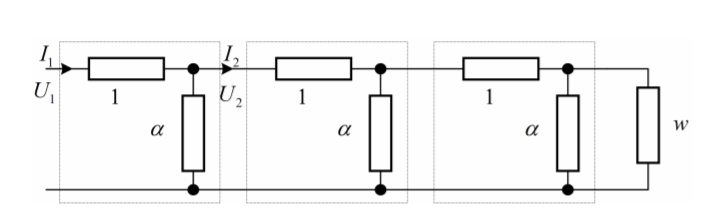
\includegraphics[width = 12 cm]{3.png}
    \caption{Лестничная структура}
    \label{fig:vac}
\end{figure}

Для напряжений и сил тока для рассматриваемой конфигурации имеем:

\begin{figure}[h!]
    \centering
    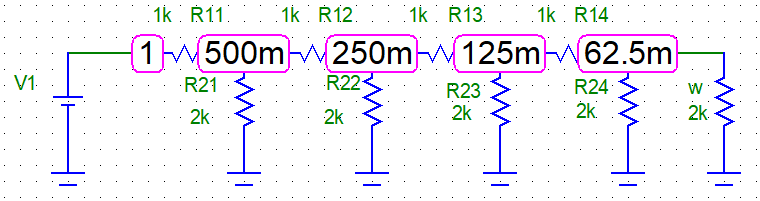
\includegraphics[width = 12 cm]{4.png}
    \caption{Напряжения лестничной структуры (1 вариант)}
    \label{fig:vac}
\end{figure}

\begin{figure}[h!]
    \centering
    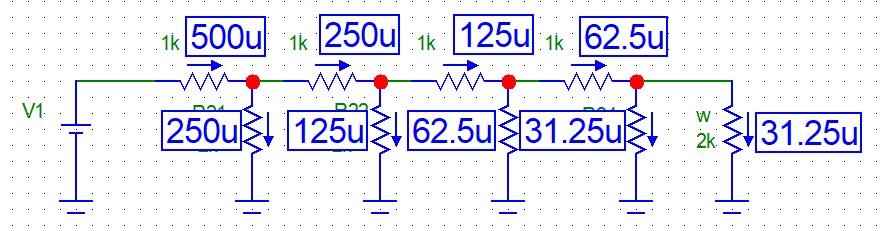
\includegraphics[width = 12 cm]{5.png}
    \caption{Силы тока лестничной структуры (1 вариант)}
    \label{fig:vac}
\end{figure}

Далее пусть $\alpha = 6$, $\gamma = 2/3$ , сопротивления $R_{2j} = 6$ кОм.

\begin{figure}[h!]
    \centering
    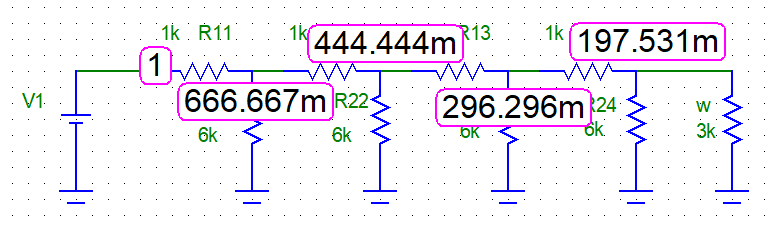
\includegraphics[width = 12 cm]{6.png}
    \caption{Напряжения лестничной структуры (2 вариант)}
    \label{fig:vac}
\end{figure}

\begin{figure}[h!]
    \centering
    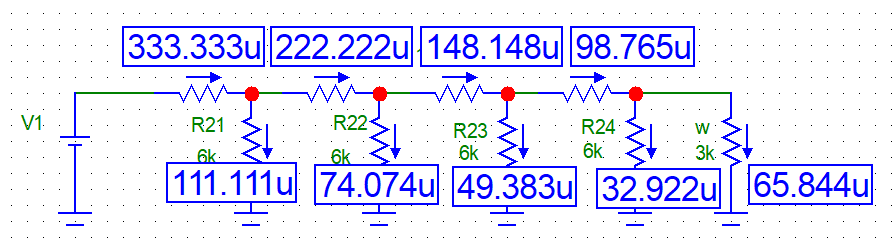
\includegraphics[width = 12 cm]{7.png}
    \caption{Силы тока лестничной структуры (2 вариант)}
    \label{fig:vac}
\end{figure}

Далее пусть $\alpha = 12$, $\gamma = 3/4$ , сопротивления $R_{2j} = 12$ кОм.

\begin{figure}[h!]
    \centering
    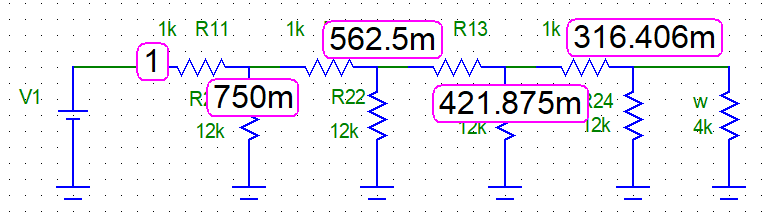
\includegraphics[width = 12 cm]{8.png}
    \caption{Напряжения лестничной структуры (3 вариант)}
    \label{fig:vac}
\end{figure}

\begin{figure}[h!]
    \centering
    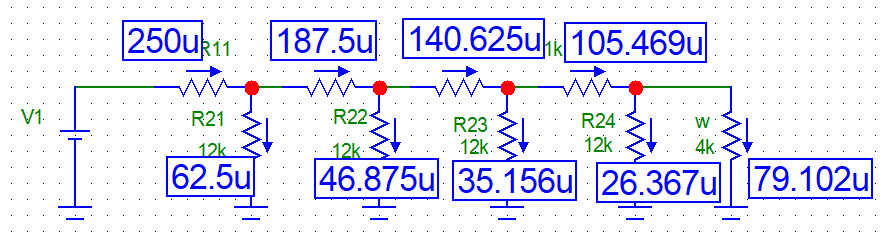
\includegraphics[width = 12 cm]{9.png}
    \caption{Силы тока лестничной структуры (3 вариант)}
    \label{fig:vac}
\end{figure}

Пусть $\alpha = 1$, $\gamma = 0.38$ , сопротивления $R_{2j} = 1$ кОм.

\begin{figure}[h!]
    \centering
    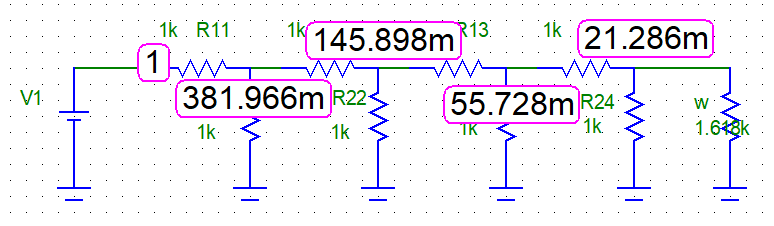
\includegraphics[width = 12 cm]{10.png}
    \caption{Напряжения лестничной структуры (4 вариант)}
    \label{fig:vac}
\end{figure}

\begin{figure}[h!]
    \centering
    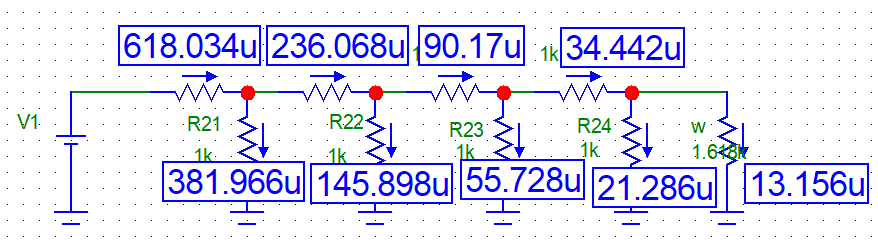
\includegraphics[width = 12 cm]{11.png}
    \caption{Силы тока лестничной структуры (4 вариант)}
    \label{fig:vac}
\end{figure}


\subsection{Исследование ЦАП}

Исследуем схему АЦП, показанную на рисунке.

\begin{table}[h!]
\centering
\begin{tabular}{|l|l|}
\hline
Число & OUT, В \\ \hline
0001  & 1      \\ \hline
0010  & 2      \\ \hline
0011  & 3      \\ \hline
0101  & 5      \\ \hline
0111  & 7      \\ \hline
1011  & 11     \\ \hline
1110  & 14     \\ \hline
\end{tabular}
\end{table}

\begin{figure}[h!]
    \centering
    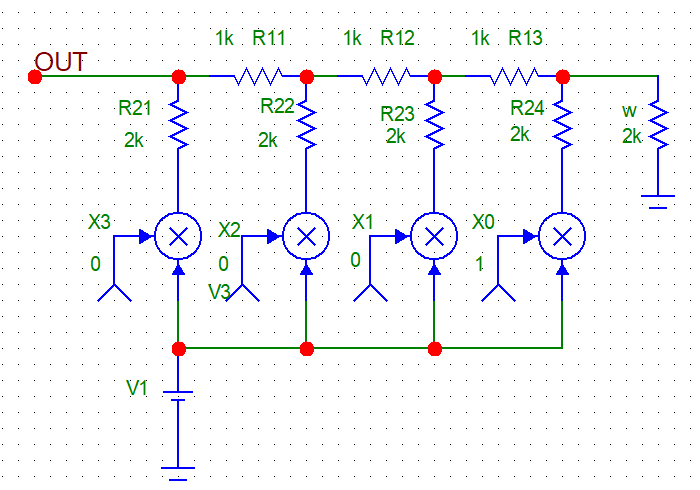
\includegraphics[width = 12 cm]{12.png}
    \caption{Схема АЦП}
    \label{fig:vac}
\end{figure}

Исследуем зависимость выходящего напряжения $OUT$ в зависимости от двоичного кода $(X1,X2,X3,X4)$.


















                    
\end{document}